\documentclass[10pt]{article}
\usepackage[a4paper,margin=20mm]{geometry}
\usepackage[T1]{fontenc}
\usepackage[utf8]{inputenc}
\usepackage{lmodern,microtype,booktabs,graphicx,hyperref}
\hypersetup{hidelinks,pdfauthor={Mathias Chebbah, Aurélien Saint-Grégoire, Ashley Russo}}
\setlength{\parindent}{0pt}\setlength{\parskip}{4pt}
\title{Supplementary analyses\\\large HABS Neuro-AI, Team 12}
\author{Mathias Chebbah \and Aurélien Saint-Grégoire \and Ashley Russo}
\date{}
\begin{document}
\maketitle
Secondary analyses of reported distress during emotional video viewing in HABS. Each section identifies its population and score. The primary classification and raw cardiac forecasting experiments are reported in the main article.
\section*{S1. Ranking viewers of the same video}
The audited four-phase Ridge model scored 12,693 development trials. Within each eligible video, its scores compared distressed and other viewers. The pair-weighted AUC was 0.5252 [0.5111, 0.5396] across 117 videos (118,663 positive--negative pairs). Against calm viewers ($V\ge5$, $A\le5$), it was 0.4918 [0.4555, 0.5336] across 37 videos (4,250 pairs); the unweighted value was 0.5243. At least three trials of each class were required per video, and intervals resample videos. These across-viewer pairs differ from those used to rank clips within an ID.

An earlier analysis reported 0.5640 [0.5276, 0.6022] on 48 videos and 6,403 pairs. It used a 10-s logistic model with global per-ID feature centering before cross-validation and a different calm definition ($V\ge5.5$, $A\le4.5$). Its higher estimate cannot isolate a perceptual or methodological mechanism. A separate within-ID physiological contrast averaged trials from clips where at least half the other trials were rated as distress. The change in HR was 2.97 bpm lower for distressed than calm trials [difference $-4.81$, $-1.10$; 26 IDs; $d=-0.41$]. Comparisons used the same ID but could involve different clips.
\section*{S2. Fear, disgust and cardiac-locked EEG}
Across trials with a first-ranked fear or disgust report, the standardized contrast is fear minus disgust within ID. The early central-parietal delta difference was $d=-0.0984$ (158 IDs). Late frontal gamma differed by $-0.1116$ (159), and its late-minus-early difference was $-0.1777$ (160); frontal muscle activity is one possible contributor. Late skin conductance differed by $+0.1929$ and late-minus-early conductance by $+0.3025$ (116 IDs). These exploratory contrasts do not hold the video fixed.

On the same R peaks, the mean distress contrast for heartbeat-evoked potentials was $d=0.0382$ [$-0.0008$, $0.0774$] in the raw branch and $0.0386$ [$-0.0021$, $0.0783$] in the ICA branch (287 IDs). Raising the raw rejection limit from 100 to 200 $\mu$V yielded $d=0.0057$. The ICA procedure did not explicitly target cardiac components. These comparisons do not test equivalence or establish the origin of information used by the forecasting model.
\section*{S3. Coherence between ratings and physiology}
We standardized variables within ID and applied PCA followed by orthogonal Varimax rotation on 16,276 complete trials. The first three components explained 53.3\% of variance. The two EDA variables loaded 0.96 on the first component and came from the same recording channel. The second component combined EEG with cardiorespiratory responses and the third included ratings. Orthogonality is a property of the rotation.

For the neuro-autonomic composite (cardiac deceleration, EDA increase, occipital alpha suppression and central-parietal delta increase), median within-ID coherence was $\rho=0.111$ (IQR 0.021--0.208; 314 IDs). In 21.0\% of IDs the estimated value was nonpositive. One-week stability was $r=0.066$ [$-0.087$, $0.211$] across 169 IDs. Finite-trial noise is compatible with these observations; its contribution is not identified. The autonomic-only composite had median $\rho=0.074$ and 28.7\% nonpositive.
\clearpage
\section*{S4. Averaging episodes of known class}
Within ID, we averaged $K$ scores sampled with replacement from trials of the same known class (200 draws per class for $K>1$). AUC measures ranking. For sensitivity only, an oracle threshold used the 90th percentile of the ID's own negative scores. Each row below shows the estimates at $K=1$ and $K=10$.
\begin{center}
\begin{tabular}{lccc}\toprule
Contrast & IDs & AUC & Sensitivity\\ \midrule
Standard & 208 & 0.569 / 0.680 & 21.0 / 41.8\,\% \\
Threat versus calm/neutral & 139 & 0.581 / 0.692 & 27.0 / 45.5\,\% \\
Strict distress versus relaxed & 147 & 0.602 / 0.698 & 31.5 / 52.8\,\% \\
\bottomrule\end{tabular}
\end{center}
Known-class averaging is an offline exercise; the trajectories are not a test of chronological alarm detection.
\begin{center}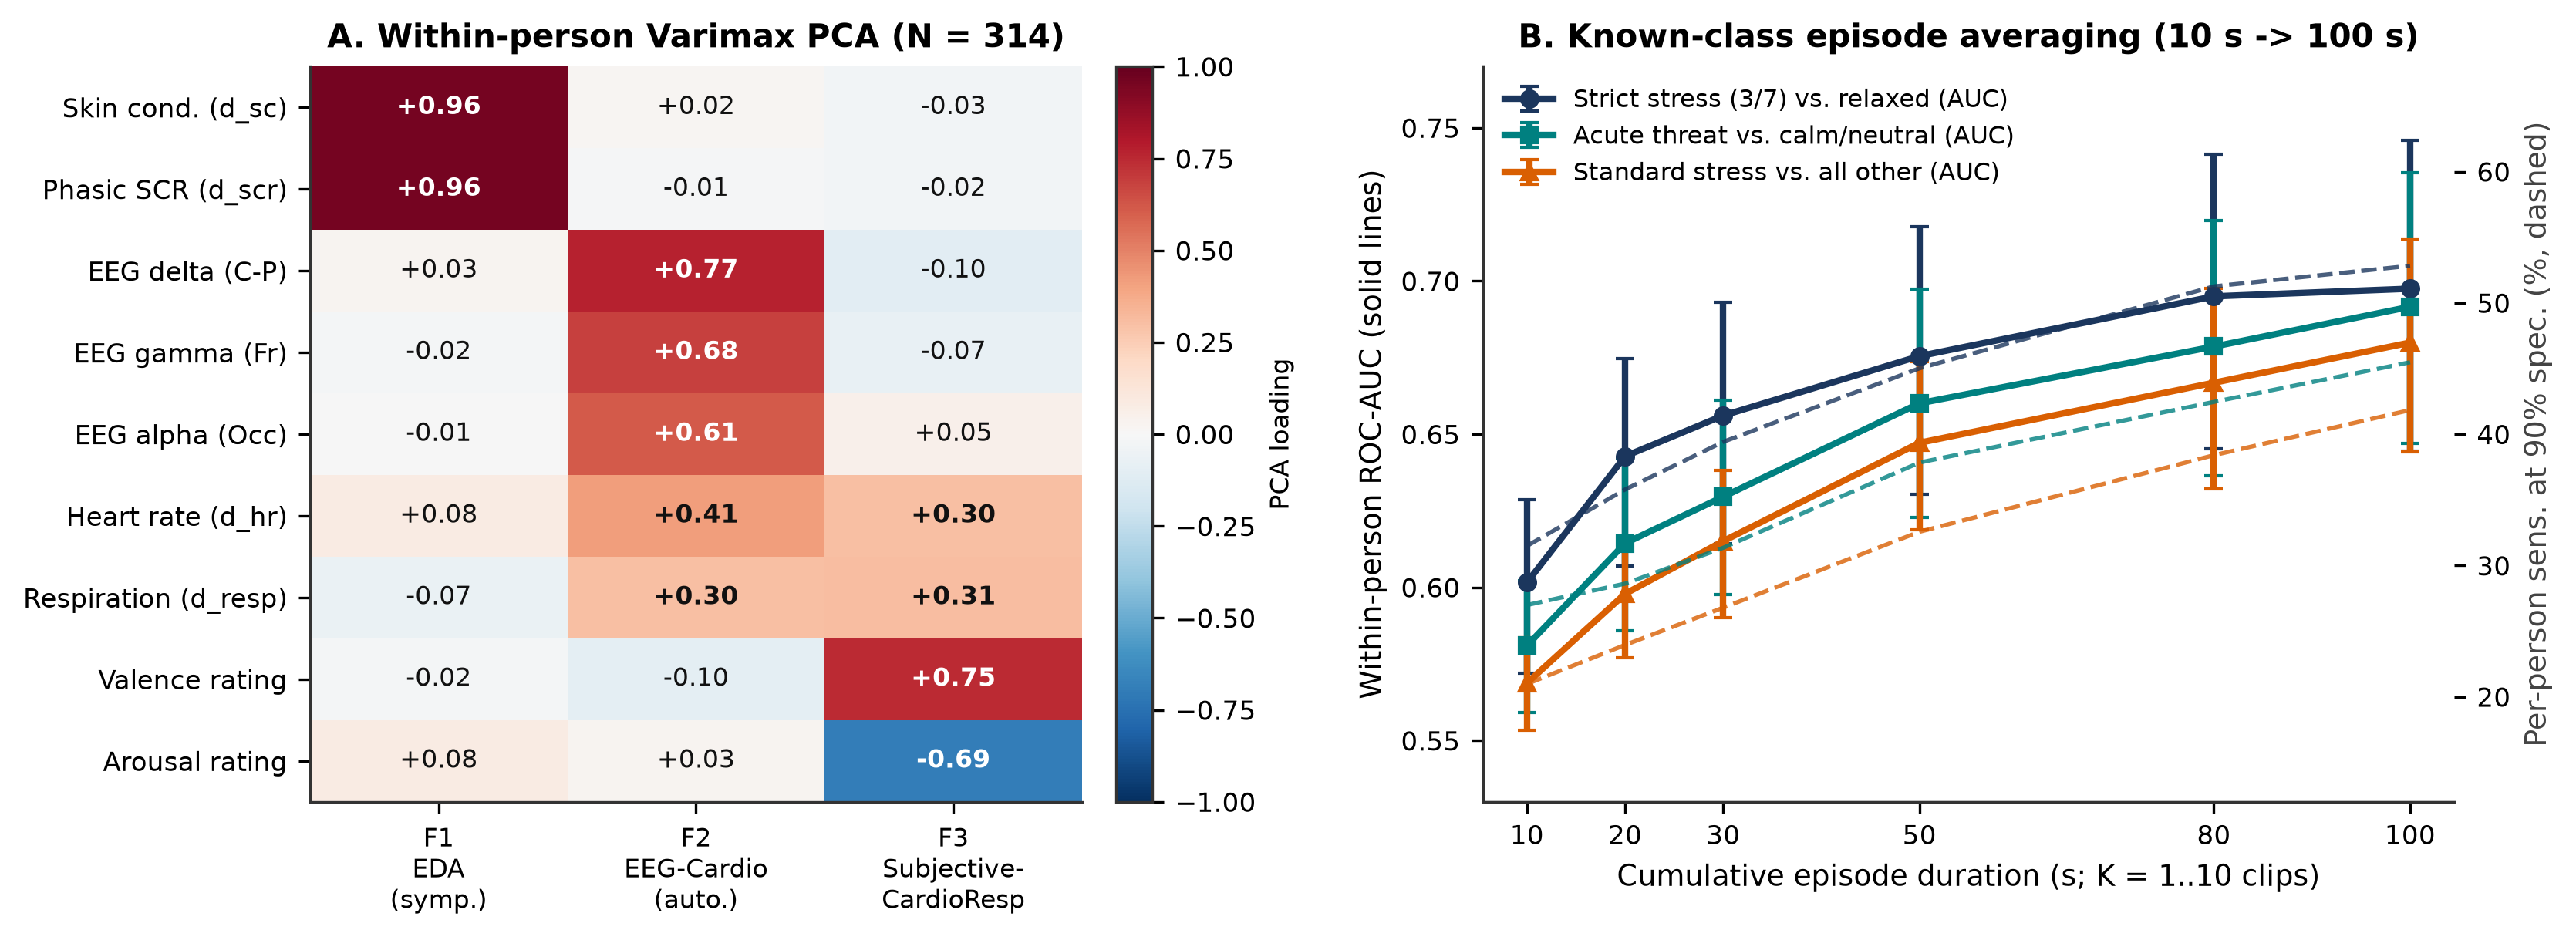
\includegraphics[width=.95\textwidth]{figures/fig4_coherence_monitoring.png}\end{center}
{\small Figure S1. Rotated PCA loadings (left) and known-class score averages (right). Lines show AUC and sensitivity at an ID-specific threshold. Disjoint blocks confirmed the standard AUC at five episodes (0.634, 148 IDs). An independent ten-episode block check was unavailable.}
\section*{S5. Transfer, adaptation and reproducibility}
In the historical one-week transfer analysis, 103 IDs were eligible on both days. Paired day-2 minus day-1 AUC was $-0.0392$ [$-0.0728$, $-0.0085$] for EDA, $+0.0246$ [$-0.0062$, $0.0548$] for engineered EEG, and $+0.0041$ [$-0.0280$, $0.0373$] for the multimodal model. Different stimulus distributions and session conditions can contribute. On a later chronological test segment, at 40 labeled calibration trials, naive personal Ridge differed from the population model by $-0.0530$ [$-0.0868$, $-0.0208$]; shrinkage toward population coefficients differed by $-0.0011$ [$-0.0264$, $0.0233$]. Unsupervised CORAL differed by $-0.0063$ [$-0.0146$, $0.0018$] (104 IDs).

The historical release-derived REVE analysis gave a positive cardiac correlation increment in all five leave-one-cohort-out folds (overall $+0.0107$ [0.0071, 0.0145]). Three cohort intervals excluded zero. The other two involved 17 and 8 IDs. This internal transfer analysis held out cohorts without a theme mask; different IDs can also represent one individual across cohorts.

The two published 5-s RMSSD correlations answer different questions. Within-ID correlation of the early and late clip phases averaged 0.2239 [0.1987, 0.2482] (313 IDs). Correlating the first 5 s of each 60-s task segment with its parent segment gave a median within-recording correlation of 0.27394 (10,263 candidate segments, 508 recordings).

\textbf{Trial index by cohort.} Out-of-fold linear AUC was 0.492 [0.458, 0.526] for C1 ($n=73$), 0.497 [0.471, 0.523] for C2 (80), 0.515 [0.457, 0.566] for C3 (16), 0.515 [0.456, 0.571] for C4 (32), and 0.544 [0.453, 0.650] for C5 (7).

\smallskip
\small\href{https://github.com/mathiaschebbah/habs/actions/runs/45854683170}{Study 11, c1eadc5}\quad\href{https://github.com/mathiaschebbah/habs/actions/runs/44635398113/attempts/2}{Figure 1A, 9dfefdf}
\quad\href{https://github.com/mathiaschebbah/habs/actions/runs/44635461916/attempts/2}{RMSSD, 9dfefdf}
\quad\href{https://github.com/mathiaschebbah/habs/actions/runs/45091493959}{Video, 9989627}
\quad\href{https://github.com/mathiaschebbah/habs/actions/runs/45604993423}{Study 10, 51394bc}
\end{document}
